% !TeX root = ../main.tex

\chapter{静态单赋值形式及其构造}
\section{从内存模型到寄存器模型}

\subsection{SSA简介}
静态单赋值形式(Static Single Assignment (SSA) form )是一种IR的实现方式,SSA由IBM实验室最早提出\cite{10.1145/73560.73562},用于编程语言和编译器设计研究中。静态单赋值要求每个变量只能被赋值一次。在SSA中,UD链(use-definechain,赋值代表define,使用变量代表use)十分明确,即每个虚拟变量都有唯一的一个define和在此define之后的use。

SSA形式对较多IR的分析,IR优化算法实现都有很大程度上的简化。例如,有如下的源代码程序:

\begin{verbatim}
    y = 1
    y = 2
    x = y
\end{verbatim}

容易观察到,第一条关于$y$的赋值语句是不必须的,它会被第二条赋值语句覆盖掉,但是我们的编译器并没有这么聪明的观察能力,基于源代码的冗余赋值语句消除需要对变量$x$和$y$进行到达定值分析,判断出$y=1$处的定值因为被$y=2$处的定值覆盖而无法到达$x=y$后,编译器才能删除第一条赋值语句。

如何基于SSA进行到达定值分析?用SSA形式描述上述代码,使用“\%”加一个唯一的数字来描述某个变量,得到的结果如下:

\begin{verbatim}
    %1 = 1
    %2 = 2
    %3 = %2
\end{verbatim}

此时不聪明的编译器也会发现,整个程序中都没有对\%1的use,这样编译器就可以简单的删去该条语句。因此,SSA形式下使用只能赋值一次的虚拟变量简化了到达定值分析。

\subsection{Memory模型SSA的介绍}

在编译器项目的前端,代码是通过 Load / Store 体系来组织的,这种SSA的组织方法被称为基于内存的静态单赋值表示(Memory-Based SSA)。

具体而言,每声明一个新变量,就通过 Store 将其存储在临时的栈帧上,当函数退出时,栈帧内的局部变量会被自动回收。当使用一个变量时,通过 Load 将其值从栈内地址读取,并赋值给一个新的变量名,之所以要给这个Load的变量取一个新名字,是为了满足SSA的单赋值要求。

给上一节的代码文件加上声明语句,使其能符合SysY的语法检查:

\begin{verbatim}
    int y;
    y = 1;
    y = 2;
    int x;
    x = y;
\end{verbatim}

那么生成的Memory SSA为:

\begin{verbatim}
    %1 = Alloca    # Allocate stack address %1
    Store %1, 1    # Store 1 into %1
    Store %1, 2    # Store 2 into %1
    %2 = Alloca    # Allocate stack address %2
    %3 = Load %1   # Load %2 into %3
    Store %3, %2   # Store %3 into %2
\end{verbatim}

这样的好处是不需要关心后端的具体实现,不牵扯到寄存器的分配问题,但是缺点同样非常明显,因为不考虑使用寄存器,所以每次使用变量之前都需要Load一次,这使得代码非常冗长且性能较低,例如在 Pentium 4架构中,基于栈式的局部变量分配的程序相比基于寄存器的局部变量分配会需要32.3\%的额外执行时间\cite{10.1145/1328195.1328197}。显然这并不适合作为竞赛用的体系架构。

\subsection{Register模型SSA的介绍}

基于寄存器的SSA是指,假定计算机有无穷多个虚拟寄存器,之前用“\%”加一个唯一的数字来描述一个单赋值虚拟变量,现在寄存器模型的SSA形式下可以理解为一个序号唯一的虚拟寄存器。

此次比赛的目标平台面向32位ARMv7,有较多个通用寄存器,因而采用寄存器模式的SSA可以有较好的效果,相比寄存于内存的SSA可以消除冗余Load或Store的次数,提高程序性能。

但是用虚拟寄存器表示SSA时,会遇到某些麻烦。考虑用IR表示一个循环的情况,那么迭代变量的值会被重复赋值,这违反了SSA的单赋值要求。

注意到迭代变量的赋值可以被划分为两种情况,第一种,刚刚经过初始化,第二种,自上次循环递增而来。在控制流程图中,这表现为迭代变量所在的基本块有两个前驱:初始化前驱和更新前驱,为了满足静态单赋值的要求,我们可以引入 $\phi$ 指令:

$\phi$指令用于根据当前基本块的执行期间的实际前驱从$\phi$指令的参数列表中选择一个值。有了$\phi$指令,就可以解决基于虚拟寄存器的SSA实现多前驱的问题,如循环体基本块Loop Block有两个前驱,且这两个前驱都对代码中的变量$x$进行了赋值,一个是初始值0,一个是更新值$x+1$,CFG表示如下:

\begin{figure}[htb]
  \centering
  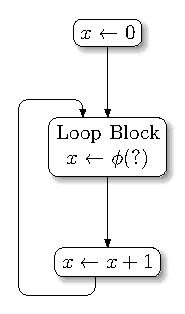
\includegraphics[width=0.3\textwidth]{figures/noSSA.pdf}
  \label{fig:nossa}
  \caption{非SSA形式的CFG}
\end{figure}


但是这显然违反了SSA的要求:对每个变量只能赋值一次。为了在不违反SSA的前提下实现循环,我们需要一种方式来重命名图中的x。

\begin{figure}[htb]
  \centering
  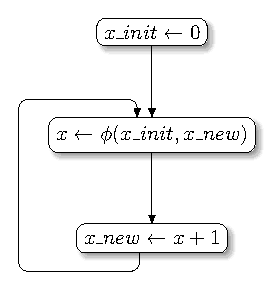
\includegraphics[width=0.4\textwidth]{figures/SSA.pdf}
  \label{fig:withssa}
  \caption{SSA形式的CFG}

\end{figure}

$\phi$指令表示,x的值取决于该指令的运行时前驱,即如果上个执行的基本块是循环初始化基本块,那么赋给x的值就是x\_init,即0;如果上个执行的基本块是循环中的更新变量基本块,那么赋值给x的就是x\_new。

\subsection{phi指令的插入位置}

从上方的例子中可以意识到,只有某个基本块的前驱数大于等于2时,才是有必要使用到$\phi$指令的,但是对于每个变量都需要一条$\phi$指令吗,这个答案是否定的,考虑图~\ref{fig:genphi}的例子(为了形象直观,这里的虚拟寄存器是采用变量加数字的形式描述,实际编译器项目中采用全局唯一的数字描述)。

\begin{figure}[htb]
  \centering
  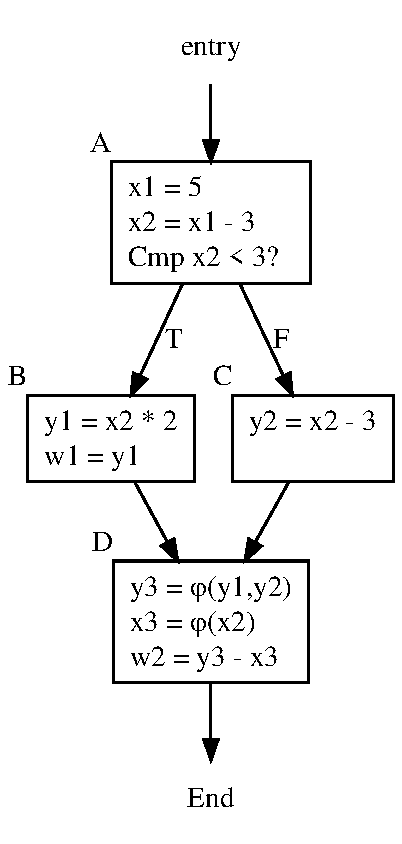
\includegraphics[width=0.4\textwidth]{figures/genphi.pdf}
  \caption{An SSA CFG Example}
  \label{fig:genphi}
\end{figure}

由该图可见,y在D中的使用,可以被指定为y1亦或是y2,这得根据它流程的来源来决定,所以插入一条关于y的$\phi$指令;但是对于x或者w,x2或w1在D中就是它们的唯一版本,即关于x或者w的$\phi$指令都只会有一个参数,因而w或x没有需要插入$\phi$指令的问题,$x3=\phi(x2)$是可以删去的。

给一个任意的控制流,如何确定哪些变量需要在哪里设置$\phi$指令?这是一个寄存器模型SSA生成中必须面对的问题,支配边界(dominance frontiers)可以有效的解决这一困难。

\section{支配关系分析} 

\subsection{什么是支配关系}

支配(Dominance)是图论中的概念:控制流图的一个节点 d 支配节点 n,当且仅当从entry节点到节点n的每一条路径均要经过节点d,写作d dom n)。

一些来相关概念:

1.说一个节点 d 严格控制节点n,当且仅当 d控制 n 而不等于 n。

2.节点 n 的立即支配节点的定义是,严格支配节点n,却不支配任何严格支配节点n的其他节点。

3. 一个节点 d 的支配边界是一个点集,其中任意节点n均满足, d 能严格支配所有节点u((u,v)是图中的一条有向边),却不能严格支配 n。支配边界就是 d 支配能力的极限。

4. 一个支配树是一棵树,它的子节点是被其立即支配的所有节点,如图~\ref{fig:domTree}。

\begin{figure}[htb]
  \centering
  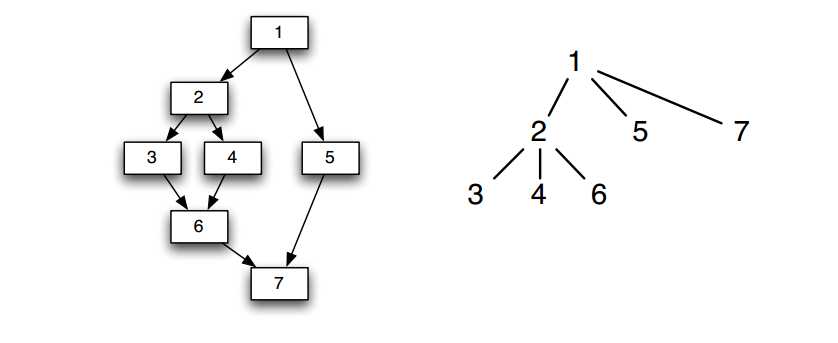
\includegraphics[width=1.0\textwidth]{figures/dom.png}
  \caption{某个CFG和对应的支配树}
  \label{fig:domTree}
\end{figure}

注:根据上述4条定义,知道了立即支配关系,连接立即支配关系下的父子节点就得到了支配树。在图~\ref{fig:domTree}中,1支配图中所有节点,因为1是全图的入口节点。2支配且立即支配3和4,同时由于6的可达路径只能为1-2-3-6或1-2-4-6,因此6被2支配但不被3或4支配,进而,2立即支配节点6,同理可得1立即支配5和7。

\subsection{支配关系分析的算法}

\subsubsection{支配关系计算}

目前求解支配树效率最高的算法是Lengauer-Tarjan algorithm \cite{10.1145/357062.357071},该算法有接近线性的复杂度,但是实现较为复杂,教学领域介绍的更多是数据流迭代求解的算法\cite{10.1145/1255450.1255452}:支配n的节点就是n和支配m的节点的并集,其中m为n的前驱。

$$
\text{DOM}(n_0)=\{n_0\}
$$

$$
\text{DOM}(n)=\{n\} \cup\left ( \mathop{\bigcap}\limits_{m \in preds(n)}  \text{DOM}(m) \right)
$$

本项目对该算法的实现伪代码可以描述为:

\begin{algorithm}[htb]
  \small
  \SetAlgoLined
  \For{each n in nodes}{
    $DOM[n] \leftarrow \{1 \cdots n\}$
    
  }
  $Changed \leftarrow True$
  
  \While{Changed}{
    $Changed \leftarrow False$
    
    \For{ each n in reversedPostOrder(nodes)}{
        $new\_set \leftarrow \{n\} \cup\left ( \mathop{\cap}\limits_{m \in preds(n)}  DOM[m] \right)$
        
        \If{$new\_set \neq DOM[n])$}{
            $Changed \leftarrow True$
            
            $DOM[n] \leftarrow new\_set$
        }
    }
  }
  \caption{The Iterative Dominator Algorithm}
  \label{algo:dom}
\end{algorithm}

该算法会初始化CFG中所有节点的支配节点为全集,然后开始按照逆后序(reverse post order)按照数据流方程更新每个节点的支配集合,直到每个节点的支配集合都不发生变化时,结束循环。

在求迭代数据流分析问题,对于该类依赖于节点前驱结果的前向数据流问题,可以对求值过程进行适当排序,使算法经过很少的迭代就能收敛,即在对当前节点n进行求值之前,应该尽量让当前节点的所有前驱节点m在本次迭代前就已经完成求值,否则会增加一次迭代过程,降低算法的效率。

这个“适当的排序”就是逆后序排序,下面对比逆后序排序和不按照逆后序排序进行遍历达到不动点需要的迭代次数,以下图为例:
\begin{figure}[htb]
  \centering
  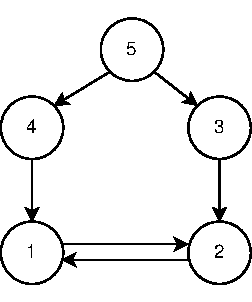
\includegraphics[width=0.3\textwidth]{figures/dom.pdf}
  \label{fig:dom}
\end{figure}

按照1-2-3-4-5的次序计算节点的支配关系,需要进行四次迭代:

\begin{table}[htb]
  \centering\small
  \caption{求图中的节点的支配关系}
  \label{tab:domcal0}
  \begin{tabular}{@{}lccccc@{}}
    \toprule
    节点   & Initial & 1st Pass & 2nd Pass & 3rd Pass & 4th Pass            \\
    \midrule
    1 &$\Omega$& \{1,2,4,5\} & \{1,4,5\} & \{1,5\} & \{1,5\} \\
    2 &$\Omega$& \{1,2,3,5\} & \{2,3,5\} & \{2,5\} & \{2,5\} \\
    3 &$\Omega$& \{3,5\} & \{3,5\} & \{3,5\} & \{3,5\} \\
    4 &$\Omega$& \{4,5\} & \{4,5\} & \{4,5\} & \{4,5\} \\
    5 &$\Omega$& \{5\} & \{5\} & \{5\} & \{5\} \\    
    \bottomrule
  \end{tabular}
\end{table}
采用逆后序遍历次序只需要进行三次迭代:

\begin{table}[htb]
  \centering\small
  \caption{按照图的逆后序遍历的节点序列求支配关系}
  \label{tab:domcal1}
  \begin{tabular}{@{}lcccc@{}}
    \toprule
    节点   & Initial & 1st Pass & 2nd Pass & 3rd Pass             \\
    \midrule
     5 & $\Omega$ & \{5\}  & \{5\} & \{5\} \\
     4 & $\Omega$ & \{5,4\} & \{5,4\} & \{5,4\} \\
     3 & $\Omega$ & \{5,3\} & \{5,3\} & \{5,3\} \\
     2 & $\Omega$ & \{5,3,2\} & \{5,2\} & \{5,2\} \\
     1 & $\Omega$ & \{5,1\} & \{5,1\} & \{5,1\} \\
        \bottomrule
  \end{tabular}
\end{table}

逆后序排序类似有向图中的拓扑排序,如果用有向图中的边表示优先级次序,头节点的优先级小于尾节点,拓扑排序要求排序结果按照优先级从高到低的顺序排列,但如果图中有环,就不可能得到一个拓扑排序结果。由于CFG中可能有环,因此逆后序排序弱化地要求尽可能多的遍历某个节点的前驱节点后再遍历该节点,这样可以减小迭代到不动点的次数。


\subsubsection{支配边界计算}

根据支配边界的定义:Y 是 X 的支配边界,当且仅当 X 支配 Y 的一个前驱结点同时 X 并不严格支配 Y。求解支配边界的算法可以用伪代码描述如下\cite{10.1145/115372.115320}:

\begin{algorithm}[htb]
  \small
  \SetAlgoLined
  \For{all b in blocks}{
    \If{b.predecessors.size() \ge 2}{
        \For{all p in b.predecessors}{
            $runner \leftarrow p$
            
            \While{runner \neq doms[b]}{
                add b to runner's dominace frontier set
                
                runner = doms[runner]
            }
        }
    }
  
  }
  \caption{The Dominance-Frontier Algorithm}
  \label{algo:domfrontier}
\end{algorithm}

该算法的描述如下:遍历所有节点,如果一个b节点的pre节点的数量少于2,那么跳入下一次循环。b节点处只有一条可达路径,不需要$\phi$指令。如果大于2,则逐个遍历节点X的pre节点,这个pre节点不是当前节点的直接支配节点,那么这个pre节点的支配边界里就要加入X节点;然后将pre节点作为当前节点,继续向前看其pre节点是否是它的直接支配节点,一直递归到前驱节点等于当前借点,或者是到达入口节点。这样,就计算出了所有BB的支配边界。

按照支配的概念,每个define必须支配对应的use(否则定值对于使用就是不可达的),所以如果达到了某个定值的支配边界基本块,就必须考虑其它路径是否有对相同变量的定值,由于在编译期间无法确定会采用哪一条分支,所以需要放置$\phi$指令来描述这种可能。


\subsection{插入phi指令}

上一节已经提到,支配边界是确定生成SSA时在何处插入必须的 $\phi$指令的解决方案。

不妨先不在乎开销,为了实现寄存器模型的SSA,最简单的方法就是,每当CFG中的节点x包含一个变量$a$的定义时,所有x的支配边界中的节点n都应该插入一条关于$a$的$\phi$指令。这种方法被称为:最小静态单赋值形式。

然而,有些 $\phi$ 函数可能会变成无用的代码,最小化SSA并不一定生产最少数量的 $\phi$ 函数。为减少 $\phi$ 函数的数量,基于以下观察:$\phi$ 函数的变量只在$\phi$ 函数所在基本块中被需要时才是必须的,即该变量在此基本块中活跃(live),因此,在插入 $\phi$ 函数的阶段,使用活跃变量信息来决定 $\phi$ 函数是否需要,只保留那些必须的$\phi$ 函数,以此方法建构剪枝的SSA。

如果为了减少分析开销和实现复杂度,可以采取折中的办法,使用半剪枝的SSA,在建构时,去掉不跨越基本块的变量名,即如果某个变量只在局部使用,就不用给它设计$\phi$ 函数。

三者的伪代码描述如下:

\begin{algorithm}[htb]
  \small
  \SetAlgoLined
  \For{all t in nodes}{
    $ S \leftarrow\{n \mid t \in \operatorname{Defs} (n)\}$

    Comupters Dominance-Frontier of n
    
    \For{all n in Dominance-Frontier}{
        Insert a $\phi$ node for t at n
    }
  }
  \caption{Inserting $\phi$ nodes (minimal SSA)}
  \label{algo:minissa}
\end{algorithm}

在最小SSA中,即为上文所提及的最简单的设置$\phi$指令的想法:在所有的有多个前驱的基本块开头对所有变量设置$\phi$指令。

\begin{algorithm}[htb]
  \small
  \SetAlgoLined
    \For{all t in nodes}{
        \If{t Lives global}{
        $ S \leftarrow\{n \mid t \in \operatorname{Defs} (n)\}$
    
        Comupters Dominance-Frontier of n
        
        \For{all n in Dominance-Frontier}{
            Insert a $\phi$ node for t at n
            
        }
    }
  }
  \caption{Inserting $\phi$ nodes (minimal SSA)}
  \label{algo:halfprunedssa}
\end{algorithm}

半剪枝的SSA只计算“全局”变量;“全局”变量是指那些在此基本块中没被赋值而被使用的,即其liveness 穿过了 Basic Block 的边界。

\begin{algorithm}[htb]
  \small
  \SetAlgoLined
    \For{all t in nodes}{
        \If{t Lives global}{
        $ S \leftarrow\{n \mid t \in \operatorname{Defs} (n)\}$
    
        Comupters Dominance-Frontier of n
        
        \For{all n in Dominance-Frontier}{
            \If{t Lives-in at n}{
            Insert a $\phi$ node for t at n
            }
        }
    }
  }
  \caption{Inserting $\phi$ nodes (pruned SSA)}
  \label{algo:prunedssa}
\end{algorithm}

剪枝的SSA不仅只计算“全局”变量,而且还需要检查在该插入关于变量t的$\phi$指令的节点n是否需要变量t,即t的定值能否到达n。

三者的对比如图~\ref{fig:why?}

\begin{figure}[htb]
  \centering
  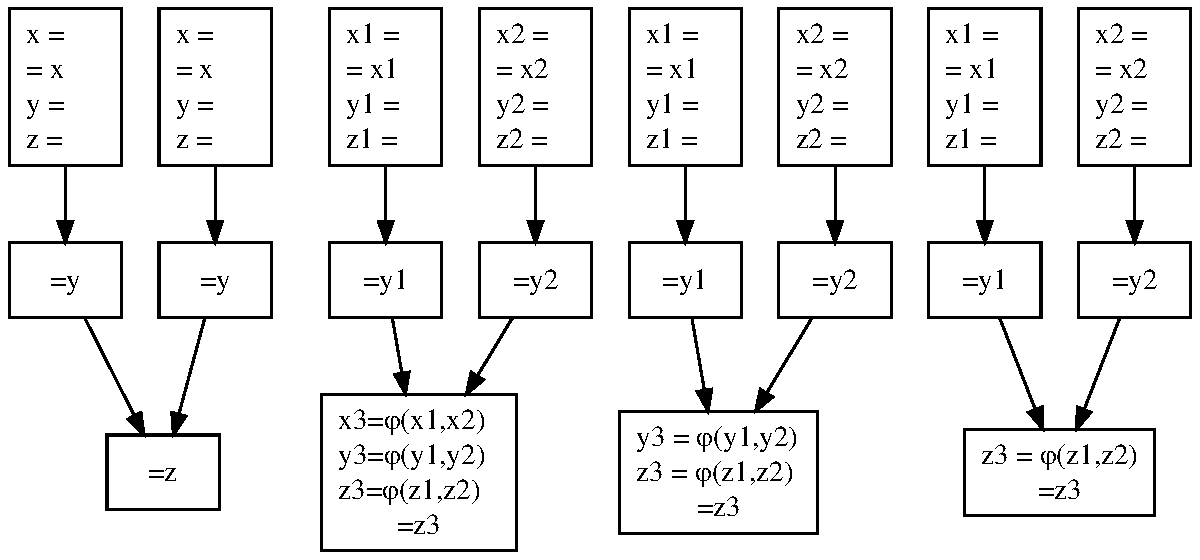
\includegraphics[width=1.0\textwidth]{figures/mini_half_pured_SSA.pdf}
  \caption{源流程图,最小SSA,半剪枝SSA,全剪枝的SSA示意图对比}
  \label{fig:why?}
  \note{注:x、y、z 为变量名,在赋值号左侧出现的变量名表示该条指令对变量进行定值,在赋值号右侧出现的变量名表示该条指令需要使用这个变量的值}
  
\end{figure}
